% SPDX-License-Identifier: CC-BY-SA-4.0
% Session: Java Memory Model
% Exercise: Linearizability

\begingroup

\begin{exercice}[Linéarisabilité]
  \label{exo:memory/linearizability}

  Quelles exécutions concurrentes sont linéarisables ?

  \begin{center}
    \scalebox{.8}{
    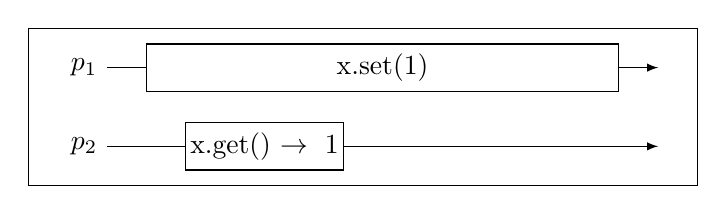
\begin{tikzpicture}
      \draw (-1,-0.5) rectangle (7.5,1.5);
      \draw[-latex] (0,1) node[left]{$p_1$} -- (7,1);
      \draw[-latex] (0,0) node[left]{$p_2$} -- (7,0);
      \draw[fill=white] (2,0) +(-1,-0.3) rectangle +(1,0.3) +(0,0) node{\lstinline{x.get()} $\rightarrow~1$};
      \draw[fill=white] (3.5,1) +(-3,-0.3) rectangle +(3,0.3) +(0,0) node{\lstinline{x.set(1)}};
    \end{tikzpicture}
    }\scalebox{.8}{
    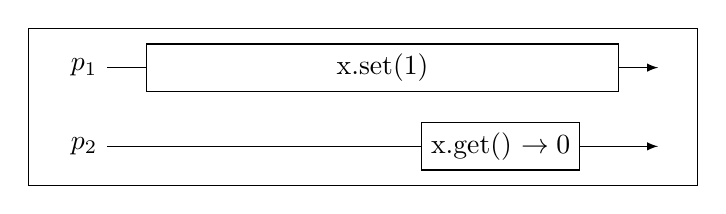
\begin{tikzpicture}
      \draw (-1,-0.5) rectangle (7.5,1.5);
      \draw[-latex] (0,1) node[left]{$p_1$} -- (7,1);
      \draw[-latex] (0,0) node[left]{$p_2$} -- (7,0);
      \draw[fill=white] (3.5,1) +(-3,-0.3) rectangle +(3,0.3) +(0,0) node{\lstinline{x.set(1)}};
      \draw[fill=white] (5,0) +(-1,-0.3) rectangle +(1,0.3) +(0,0) node{\lstinline{x.get()} $\rightarrow 0$};
    \end{tikzpicture}
    }
    
    \vspace{3mm}
    \scalebox{.8}{
    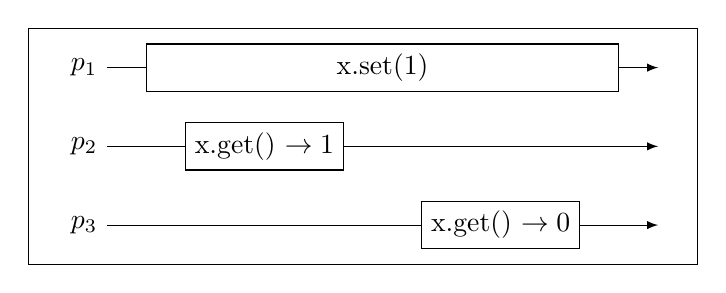
\begin{tikzpicture}
      \draw (-1,-1.5) rectangle (7.5,1.5);
      \draw[-latex] (0,1) node[left]{$p_1$} -- (7,1);
      \draw[-latex] (0,0) node[left]{$p_2$} -- (7,0);
      \draw[-latex] (0,-1) node[left]{$p_3$} -- (7,-1);
      \draw[fill=white] (2,0) +(-1,-0.3) rectangle +(1,0.3) +(0,0) node{\lstinline{x.get()} $\rightarrow 1$};
      \draw[fill=white] (3.5,1) +(-3,-0.3) rectangle +(3,0.3) +(0,0) node{\lstinline{x.set(1)}};
      \draw[fill=white] (5,-1) +(-1,-0.3) rectangle +(1,0.3) +(0,0) node{\lstinline{x.get()} $\rightarrow 0$};
    \end{tikzpicture}
    }\scalebox{.8}{
    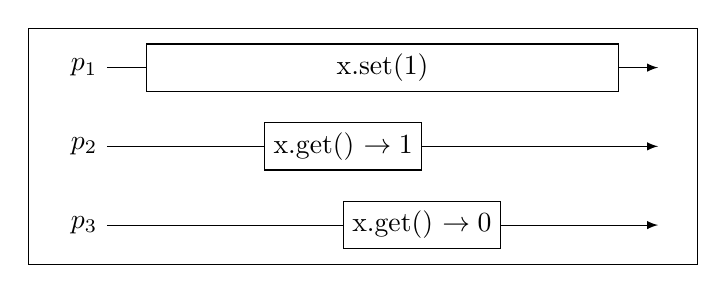
\begin{tikzpicture}
      \draw (-1,-1.5) rectangle (7.5,1.5);
      \draw[-latex] (0,1) node[left]{$p_1$} -- (7,1);
      \draw[-latex] (0,0) node[left]{$p_2$} -- (7,0);
      \draw[-latex] (0,-1) node[left]{$p_3$} -- (7,-1);
      \draw[fill=white] (3,0) +(-1,-0.3) rectangle +(1,0.3) +(0,0) node{\lstinline{x.get()} $\rightarrow 1$};
      \draw[fill=white] (3.5,1) +(-3,-0.3) rectangle +(3,0.3) +(0,0) node{\lstinline{x.set(1)}};
      \draw[fill=white] (4,-1) +(-1,-0.3) rectangle +(1,0.3) +(0,0) node{\lstinline{x.get()} $\rightarrow 0$};
    \end{tikzpicture}
    }
    
    \vspace{3mm}
    \scalebox{.8}{
    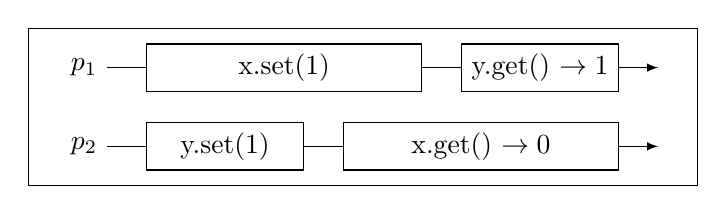
\begin{tikzpicture}
      \draw (-1,-0.5) rectangle (7.5,1.5);
      \draw[-latex] (0,1) node[left]{$p_1$} -- (7,1);
      \draw[-latex] (0,0) node[left]{$p_2$} -- (7,0);
      \draw[fill=white] (2.25,1) +(-1.75,-0.3) rectangle +(1.75,0.3) +(0,0) node{\lstinline{x.set(1)}};
      \draw[fill=white] (5.5,1) +(-1,-0.3) rectangle +(1,0.3) +(0,0) node{\lstinline{y.get()} $\rightarrow 1$};
      \draw[fill=white] (1.5,0) +(-1,-0.3) rectangle +(1,0.3) +(0,0) node{\lstinline{y.set(1)}};
      \draw[fill=white] (4.75,0) +(-1.75,-0.3) rectangle +(1.75,0.3) +(0,0) node{\lstinline{x.get()} $\rightarrow 0$};
    \end{tikzpicture}
    }\scalebox{.8}{
    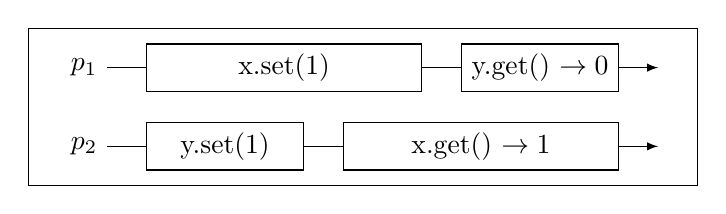
\begin{tikzpicture}
      \draw (-1,-0.5) rectangle (7.5,1.5);
      \draw[-latex] (0,1) node[left]{$p_1$} -- (7,1);
      \draw[-latex] (0,0) node[left]{$p_2$} -- (7,0);
      \draw[fill=white] (2.25,1) +(-1.75,-0.3) rectangle +(1.75,0.3) +(0,0) node{\lstinline{x.set(1)}};
      \draw[fill=white] (5.5,1) +(-1,-0.3) rectangle +(1,0.3) +(0,0) node{\lstinline{y.get()} $\rightarrow 0$};
      \draw[fill=white] (1.5,0) +(-1,-0.3) rectangle +(1,0.3) +(0,0) node{\lstinline{y.set(1)}};
      \draw[fill=white] (4.75,0) +(-1.75,-0.3) rectangle +(1.75,0.3) +(0,0) node{\lstinline{x.get()} $\rightarrow 1$};
    \end{tikzpicture}
    }
  \end{center}
\end{exercice}

\endgroup
\endinput
